\documentclass[12pt,a4paper]{article}
\usepackage{ctex}
\usepackage{amsmath,amscd,amsbsy,amssymb,latexsym,url,bm,amsthm}
\usepackage{epsfig,graphicx,subfigure}
\usepackage{enumitem,balance}
\usepackage{wrapfig}
\usepackage{mathrsfs,euscript}
\usepackage[usenames]{xcolor}
\usepackage{hyperref}
\usepackage[vlined,ruled,linesnumbered]{algorithm2e}
\hypersetup{colorlinks=true,linkcolor=black}

\newtheorem{theorem}{Theorem}
\newtheorem{lemma}[theorem]{Lemma}
\newtheorem{proposition}[theorem]{Proposition}
\newtheorem{corollary}[theorem]{Corollary}
\newtheorem{exercise}{Exercise}
\newtheorem*{solution}{Solution}
\newtheorem{definition}{Definition}
\theoremstyle{definition}

\renewcommand{\thefootnote}{\fnsymbol{footnote}}

\newcommand{\postscript}[2]
 {\setlength{\epsfxsize}{#2\hsize}
  \centerline{\epsfbox{#1}}}

\renewcommand{\baselinestretch}{1.0}

\setlength{\oddsidemargin}{-0.365in}
\setlength{\evensidemargin}{-0.365in}
\setlength{\topmargin}{-0.3in}
\setlength{\headheight}{0in}
\setlength{\headsep}{0in}
\setlength{\textheight}{10.1in}
\setlength{\textwidth}{7in}
\makeatletter \renewenvironment{proof}[1][Proof] {\par\pushQED{\qed}\normalfont\topsep6\p@\@plus6\p@\relax\trivlist\item[\hskip\labelsep\bfseries#1\@addpunct{.}]\ignorespaces}{\popQED\endtrivlist\@endpefalse} \makeatother
\makeatletter
\renewenvironment{solution}[1][Solution] {\par\pushQED{\qed}\normalfont\topsep6\p@\@plus6\p@\relax\trivlist\item[\hskip\labelsep\bfseries#1\@addpunct{.}]\ignorespaces}{\popQED\endtrivlist\@endpefalse} \makeatother

\begin{document}
\noindent

%========================================================================
\noindent\framebox[\linewidth]{\shortstack[c]{
\Large{\textbf{Lab05-Amortized Analysis}}\vspace{1mm}\\
CS214-Algorithm and Complexity, Xiaofeng Gao, Spring 2018.}}
\begin{center}

\footnotesize{\color{blue}$*$ Name: Hongyi Guo  \quad Student ID: 516030910306 \quad Email: guohongyi@sjtu.edu.cn}
\end{center}

\begin{enumerate}
\item A \textbf{multistack} consists of an infinite series of stacks $S_0, S_1, S_2,\cdots$, where the $i^{th}$ stack $S_i$ can hold up to $3^i$ elements. Whenever a user attempts to push an element onto any full stack $S_i$, we first pop all the elements off $S_i$ and push them onto stack $S_{i+1}$ to make room. (Thus, if $S_{i+1}$ is already full, we first recursively move all its members to $S_{i+2}$.) An illustrative example is shown in Figure \ref{Fig-MultiStack}. Moving a single element from one stack to the next takes $O(1)$ time. If we push a new element, \underline{we always intend to push it in stack $S_0$}.

\begin{figure}[!htbp]
\centering
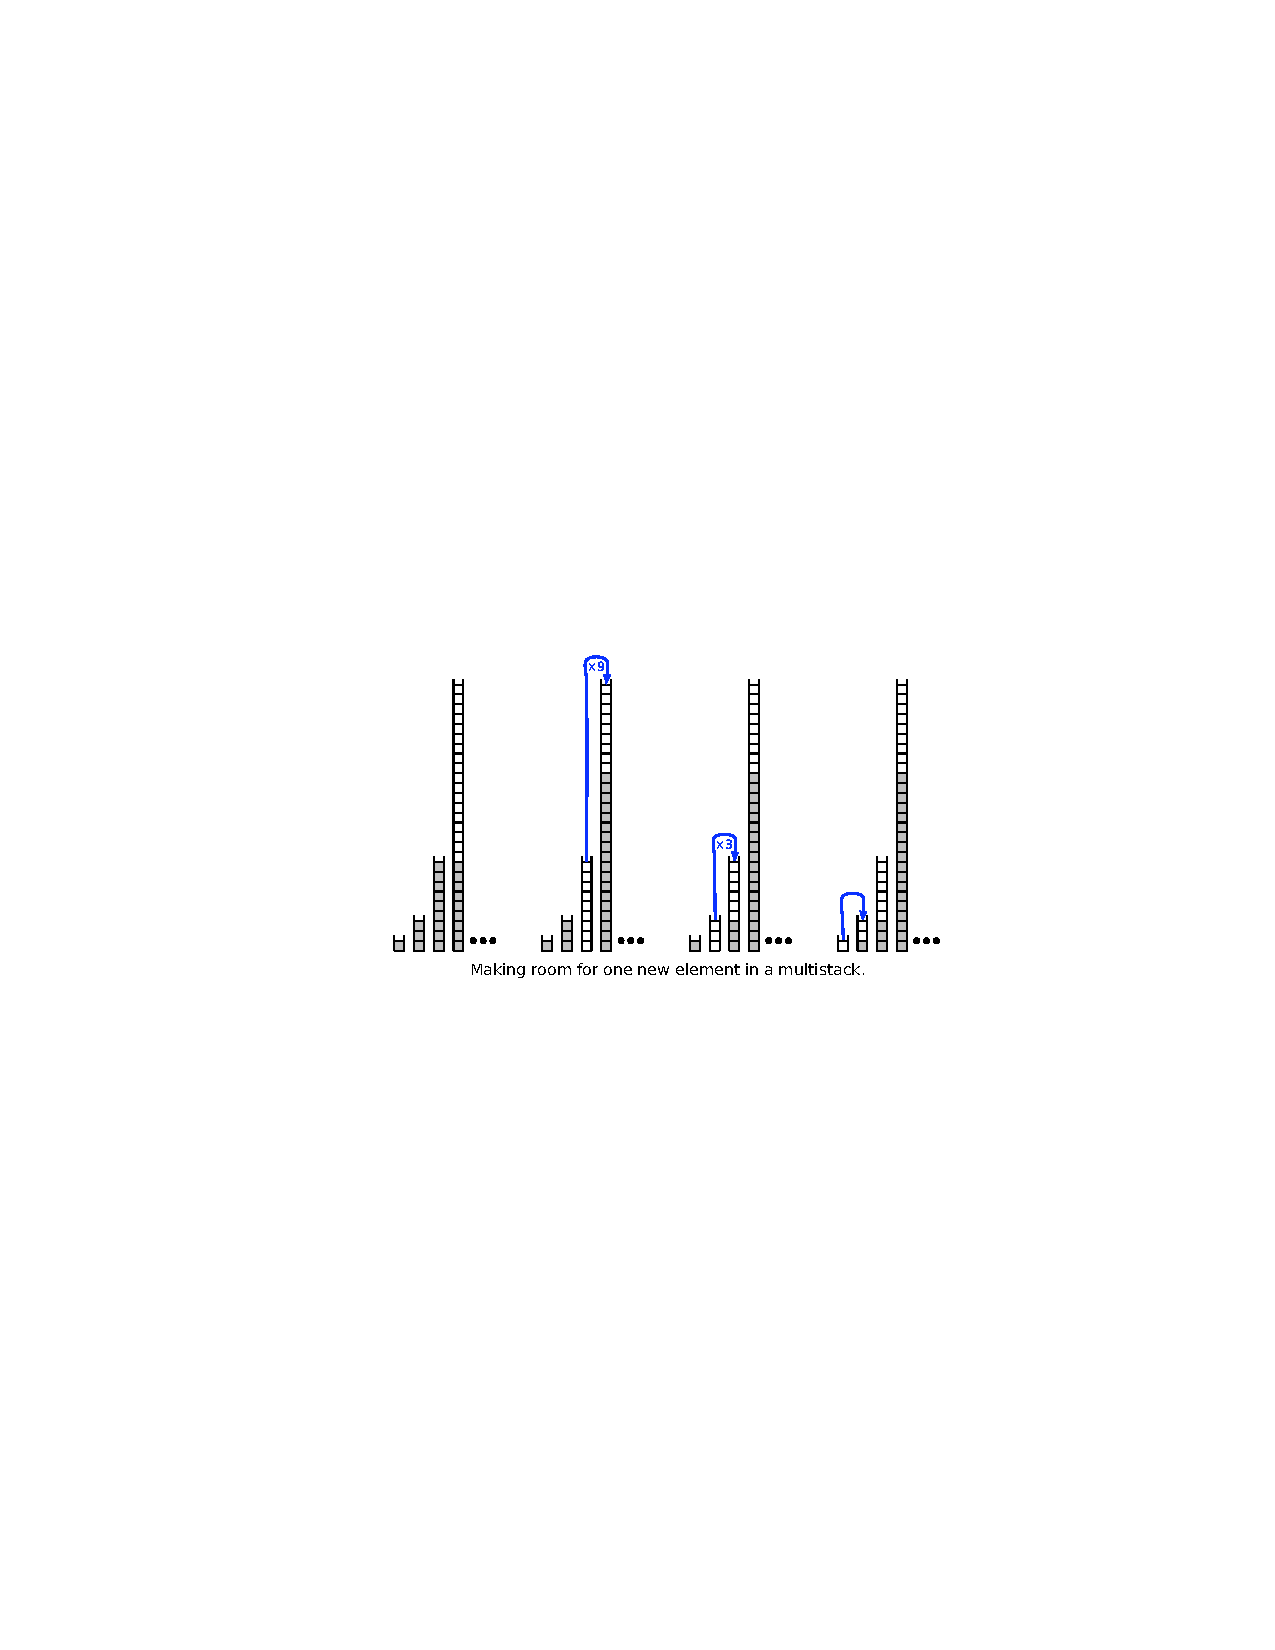
\includegraphics[width=0.5\textwidth]{Fig-MultiStack.pdf}
\caption{An example of making room for one new element in a multistack.}
\label{Fig-MultiStack}
\end{figure}

    \begin{enumerate}
        \item In the worst case, how long does it take to push a new element onto a multistack containing $n$ elements?
        
        \begin{solution}
        	When $n=1+\sum_{i=0}^{k}3^i$, all non-empty stacks are already full. Each element needs to be popped and pushed into its next stack. So, it's the worst case, and it takes $T(n)=n$.
        	
        \end{solution}
    
        \item Prove that the amortized cost of a push operation is $O(\log n)$ by \emph{Aggregation Analysis}.
        
        \begin{solution}
        	We denote the total time of inserting $n$ elements by $S_n$. Notice that the $S_n$ is no worse than when the $n^{th}$ insert is in its worst case, as to say, $n=1+\sum_{i=0}^{k}3^i$. So,
        	\begin{equation}
        		S_n\leq 1+1*3^0+2*3^1+3*3^2+\dots+(k+1)*3^k
        	\end{equation}
        	where, 
        	$$
        	n\leq 1+(1+3+3^2+\dots+3^k)=\frac{3^{k+1}+1}{2}
        	$$        	
        	So, 
        	$$
        	k+1\geq \log_3(2n-1)$$ and $$k<\log_3(2n-1)
        	$$
        	Then we compute $S_n$.
        	\begin{equation}
        		3*S_n=3+1*3^1+2*3^2+3*3^3+\dots+k*3^k+(k+1)*3^{k+1}
        	\end{equation}
        	(2)$-$(1), we get 
        	$$
        	2*S_n=1-3-3^2-\dots-3^k+(k+1)*3^{k+1}=\frac{(2k+1)*3^{k+1}+5}{2}
        	$$
        	Thus, the amortized cost of a push operation is
        	$$\frac{S_n}{n}=\frac{(2k+1)*3^{k+1}+5}{4n}=\frac{6k+3}{4}*\frac{2n-1}{n}+\frac{5}{4n}=O(k)=O(\log_3(2n-1))=O(\log n)$$
        	
        \end{solution}
    
        \item {\color{red}(Optional Subquestion with Bonus)} Prove that the amortized cost of a push operation is $O(\log n)$ by \emph{Potential Method}.
        
        \begin{solution}
        	Assign
        	$$
        	\Phi(i)=\begin{cases}
        	k\log n- weight_i\nonumber,\quad i>0\\
        	0,\quad\quad\quad\quad\quad\quad\quad\quad i=0
        	\end{cases}
        	$$
        	I assign a weight $\sum_{j=1}^{k_i}j*|S_j|$ to each state, where $k_i$ is the number of non-empty stacks, say the state is just after the $i^{th}$ insertion. So, $c_i=weight_i-weight_{i-1}$. Due to the definition of $weight_i$, we know for $i>0$, $weight_i\leq \log n+\log n+\dots+\log n = k_i\log n$. So $\Phi(i)\geq 0$. Note that $\Phi(0)=0$. Thus, $\Phi(n)\geq\Phi(0)$.
        	
        	When we insert the $i^{th}$ element, the times of push and pops are $weight_i-weight_{i-1}$. 
        	$$
        	\hat{c_i} = c_i+\Phi(i)-\Phi(i-1)=c_i+k_i\log n+k_{i-1}\log n-(weight_i-weight_{i-1}) = (k_i-k_{i-1})\log n\leq\log n
        	$$
        	So, the amortized cost of a push operation is $O(\log n)$.
        \end{solution}
    \end{enumerate}

\item A factory needs to deliver a kind of product in $2$ months. Suppose that for month $i$: the contract requires the factory to deliver $d_i$ products; the selling price for a product is $s_{i}$; the capitalized cost for a product is $c_{i}$; the working time needed for a product is $t_{i}$. In month $i$, the normal working time is no more than $T_{i}$, and it is allowed to do extra work, but the extra working time is no more than $T_{i}^{\prime}$, and each product produced in extra working time has an extra $c_{i}^{\prime}$ in its capitalized cost. If the products are stored (not delivered) in month $i$, the storage cost $p_i$ is required to pay for each stored product.

Please design a production plan in the form of linear programming, which maximizes the overall profit under all possible constraints mentioned above.

\begin{enumerate}
\item  Please add some necessary explanations on your objective function and constraints, and finally write your LP in \emph{standard} form.

\begin{solution} Suppose in month $i$, we produce $a_i$ products within normal working time and $b_i$ in extra working time. So, we have objective function as following
	$$
	\text{max}\quad\quad\quad\sum_{i=1}^{2}\left[(a_i+b_i)s_i - b_i(c_i+c_i') - a_ic_i - (a_i+b_i-d_i)p_i\right]
	$$
	The overall profit is equal to total income $(a_i+b_i)s_i$ minus total cost which is divided into three parts, working time cost $a_ic_i$, extra time cost $b_i(c_i+c_i')$ and storage cost $(a_i+b_i-d_i)p_i$.
	
	The constrains are as following
	\begin{equation}
	\begin{aligned}
	a_i+b_i&\geq d_i\quad(i=1,2)\\
	a_it_i &\leq T_i\quad(i=1,2)\\
	b_it_i &\leq T_i'\quad(i=1,2)\\
	a_i,b_i&\geq 0\quad(i=1,2)\\	
	\end{aligned}\nonumber
	\end{equation}
	
	Obviously, $a_i$ and $b_i$ are all non-negative integers, and their sum must be greater or equal to $d_i$ to satisfy the delivery demands. Then time consumed by producing in working time cannot exceed $T_i$ and time consumed by producing in extra working time cannot exceed $T_i'$. So we get the constrains above.
	
	The nature form:
	$$
	\text{max}\quad\quad\quad\sum_{i=1}^{2}\left[(s_i-c_i-p_i)a_i+(s_i-c_i-c_i'-p_i)b_i+p_id_i\right]
	$$
	\begin{equation}
	\begin{aligned}
	-a_i-b_i&\leq -d_i\quad(i=1,2)\\
	a_i     &\leq T_i/t_i\quad(i=1,2)\\
	b_i     &\leq T_i'/t_i\quad(i=1,2)\\
	a_i,b_i &\geq 0\quad(i=1,2)\\
	\end{aligned}\nonumber
	\end{equation}
	
\end{solution}
\item Transform your LP into its dual form.

\begin{solution}
	$$
	\text{min}\quad\quad\quad\sum_{i=1}^{2}\left[-d_i\alpha_i + (T_i/t_i)\beta_i + (T_i'/t_i)\gamma_i + p_id_i\right]
	$$
	\begin{equation}
	\begin{aligned}
	-\alpha_i+\beta_i &\geq s_i-c_i-p_i\quad(i=1,2)\\
	-\alpha_i+\gamma_i&\geq s_i-c_i-c_i'-p_i\quad(i=1,2)\\
	\alpha_i, \beta_i,\gamma_i & \geq 0\quad(i=1,2)\\
	\end{aligned}\nonumber
	\end{equation}
\end{solution}
\end{enumerate}

\end{enumerate}

\textbf{Remark:} Please include .pdf and  .tex files in your .rar or .zip file with standard file names.

%========================================================================
\end{document}
